% Options for packages loaded elsewhere
\PassOptionsToPackage{unicode}{hyperref}
\PassOptionsToPackage{hyphens}{url}
%
\documentclass[
]{book}
\title{Drumlogs}
\author{Isaac Medina}
\date{2023-07-16}

\usepackage{amsmath,amssymb}
\usepackage{lmodern}
\usepackage{iftex}
\ifPDFTeX
  \usepackage[T1]{fontenc}
  \usepackage[utf8]{inputenc}
  \usepackage{textcomp} % provide euro and other symbols
\else % if luatex or xetex
  \usepackage{unicode-math}
  \defaultfontfeatures{Scale=MatchLowercase}
  \defaultfontfeatures[\rmfamily]{Ligatures=TeX,Scale=1}
\fi
% Use upquote if available, for straight quotes in verbatim environments
\IfFileExists{upquote.sty}{\usepackage{upquote}}{}
\IfFileExists{microtype.sty}{% use microtype if available
  \usepackage[]{microtype}
  \UseMicrotypeSet[protrusion]{basicmath} % disable protrusion for tt fonts
}{}
\makeatletter
\@ifundefined{KOMAClassName}{% if non-KOMA class
  \IfFileExists{parskip.sty}{%
    \usepackage{parskip}
  }{% else
    \setlength{\parindent}{0pt}
    \setlength{\parskip}{6pt plus 2pt minus 1pt}}
}{% if KOMA class
  \KOMAoptions{parskip=half}}
\makeatother
\usepackage{xcolor}
\IfFileExists{xurl.sty}{\usepackage{xurl}}{} % add URL line breaks if available
\IfFileExists{bookmark.sty}{\usepackage{bookmark}}{\usepackage{hyperref}}
\hypersetup{
  pdftitle={Drumlogs},
  pdfauthor={Isaac Medina},
  hidelinks,
  pdfcreator={LaTeX via pandoc}}
\urlstyle{same} % disable monospaced font for URLs
\usepackage{longtable,booktabs,array}
\usepackage{calc} % for calculating minipage widths
% Correct order of tables after \paragraph or \subparagraph
\usepackage{etoolbox}
\makeatletter
\patchcmd\longtable{\par}{\if@noskipsec\mbox{}\fi\par}{}{}
\makeatother
% Allow footnotes in longtable head/foot
\IfFileExists{footnotehyper.sty}{\usepackage{footnotehyper}}{\usepackage{footnote}}
\makesavenoteenv{longtable}
\usepackage{graphicx}
\makeatletter
\def\maxwidth{\ifdim\Gin@nat@width>\linewidth\linewidth\else\Gin@nat@width\fi}
\def\maxheight{\ifdim\Gin@nat@height>\textheight\textheight\else\Gin@nat@height\fi}
\makeatother
% Scale images if necessary, so that they will not overflow the page
% margins by default, and it is still possible to overwrite the defaults
% using explicit options in \includegraphics[width, height, ...]{}
\setkeys{Gin}{width=\maxwidth,height=\maxheight,keepaspectratio}
% Set default figure placement to htbp
\makeatletter
\def\fps@figure{htbp}
\makeatother
\setlength{\emergencystretch}{3em} % prevent overfull lines
\providecommand{\tightlist}{%
  \setlength{\itemsep}{0pt}\setlength{\parskip}{0pt}}
\setcounter{secnumdepth}{5}
\usepackage{booktabs}
\usepackage[utf8]{inputenc}
\usepackage[german]{babel}
\ifLuaTeX
  \usepackage{selnolig}  % disable illegal ligatures
\fi
\usepackage[]{natbib}
\bibliographystyle{plainnat}

\begin{document}
\maketitle

{
\setcounter{tocdepth}{1}
\tableofcontents
}
\hypertarget{section}{%
\chapter*{}\label{section}}
\addcontentsline{toc}{chapter}{}

\begin{center}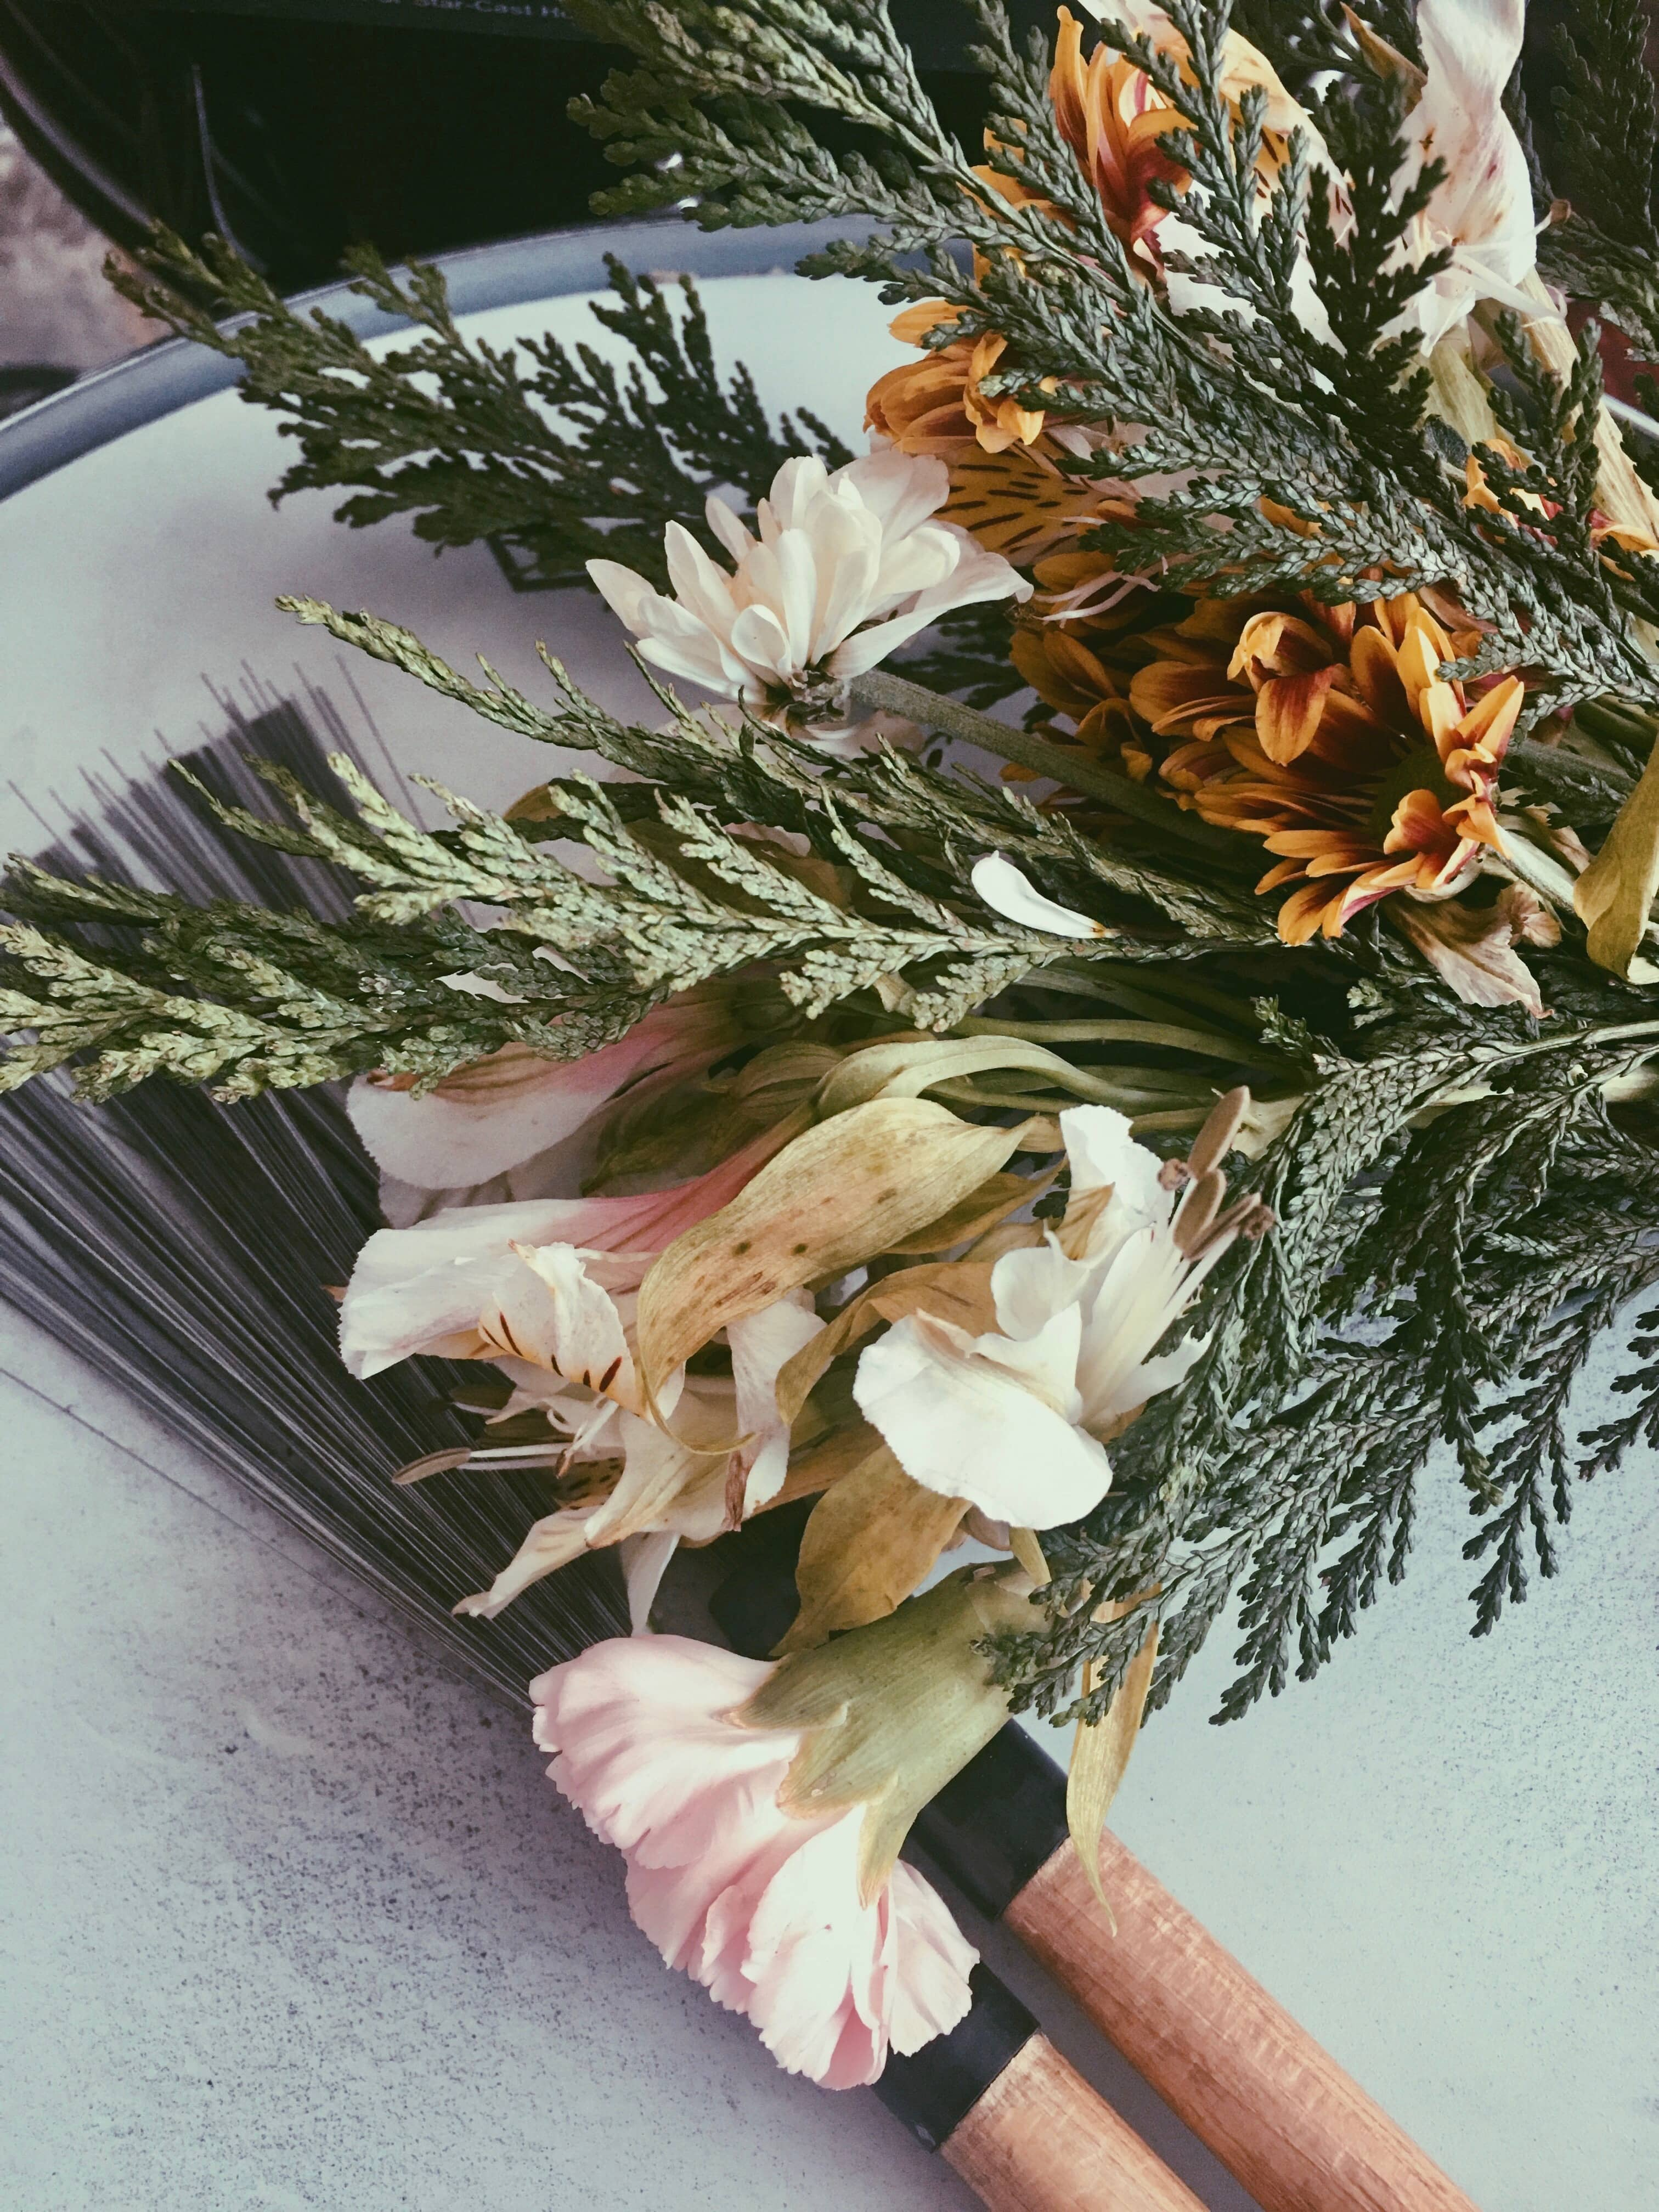
\includegraphics[width=0.6\linewidth]{images/flowerBrush1} \end{center}

\hypertarget{yes-im-a-drummer}{%
\section*{Yes, i'm a drummer}\label{yes-im-a-drummer}}
\addcontentsline{toc}{section}{Yes, i'm a drummer}

And this is my \protect\hyperlink{Diary}{Diary}. Well, sort of, mainly because there are times when logs just don't make it till here. Anyways, this webpage is an effort to keep you up to date on what i'm up to regarding drums and also a timeline to help me remember where i've been and my interests from day to day.

Yes, i'm a drummer but also teacher, synth freak, artist, friend, lover and son, that's why things here are personal, though at times it all may seem very technical. That's an advice to you while also a note for me, because the way i do things will probably not apply to many out there and won't necessarily make you/me the fastest, heaviest or even funkiest drummer, the activities recorded here are just a way of being.

Be very welcomed into this digital book, refer to \protect\hyperlink{Express-rhythm}{Express rhythm} to find further information on rhythms written with words or code, and click on \protect\hyperlink{About}{About} to check out my short bio and contact links. Have a pleasant day!

Isaac Medina

\hypertarget{Diary}{%
\chapter{Diary}\label{Diary}}

\begin{center}\rule{0.5\linewidth}{0.5pt}\end{center}

\hypertarget{juli-2023}{%
\section*{Juli 2023}\label{juli-2023}}
\addcontentsline{toc}{section}{Juli 2023}

Sa 15. \emph{Konzert}, recital de Leipzig. Todo resultó en orden y puntual. La batería fue amplificada con un micrófono de lápiz como overhead y un micrófono dinámico al bombo, Moongel en tarola, cobijas en bombo. Llegué media hora tarde, ensamblé la batería en 20 minutos con reacomodos.

Mo 11. \emph{The Art of Bop Drumming}, Comp Example 2, lick 9 with tumbao, inverted doubles and clave.

So 09. \emph{The Breakbeat Bible}, Funky Drummer @ 80-84, 6-8 Minute reps.

Sa 08. \emph{Paradiddle Johnnie}, review till bar 32, practice pad.

Mi 05. \emph{Gedanken}, ¿Cómo nos acercamos a una canción?: Instrumentación, Pulso, Ritmo, Estructura, Interpretación.

\hypertarget{juni-2023}{%
\section*{Juni 2023}\label{juni-2023}}
\addcontentsline{toc}{section}{Juni 2023}

Mo 26. \emph{The Art of Bop Drumming}, Comp Example 2, licks 5 \& 6, playing triplets as 16th notes in groups of inverted doubles \texttt{e\ \&} and placing 8ths on the last 16th \texttt{a}. Steady \emph{tumbao} on bass drum.

\hypertarget{jun262023}{}

Di 20. \emph{The Art of Bop Drumming}, some excercises over Rumba Clave.

So 18. \emph{Concert}, Vi a Horacio ``El Negro'' Hernández en Jazzatlán. El timbalero tocó desde mi perspectiva en momentos muy fuerte y con frases forzadas.

Do 15. \emph{Can't Take My Eyes Off You}, transcription till chorus.

Sa 17. \emph{Paradiddle Johnnie}, bars 1-24 on practice pad, @ 70 BPM.

Di 13. \emph{Coding}, practice of Jungle beats with Tidalcycles for the upcoming Algorave event.

Do 08. \emph{Paradiddle Johnnie}, bars 1-16, shuffle feel, various orchestrations (toms, hi-hat, snare).

So 04. \emph{The Breakbeat Bible, E6: Syncopated Accents on the Snare}, ex 1-4 with inverted doubles. \emph{Improv}. \textbf{40 min}

Fr 02. \emph{Paradiddle Johnnie}, bars 1-16, shuffle feel, accents reinforced on Bassdrum, sticks and brushes.

\hypertarget{mai-2023}{%
\section*{Mai 2023}\label{mai-2023}}
\addcontentsline{toc}{section}{Mai 2023}

Mo 29. \emph{The All American Drummer}, Solo 14 @ 50 and 60 BPM. \emph{Take Me Out, Franz Ferdinand}, weiter bearbeitet, decided to use ligatures for open Hi-Hats as it is more explicit and \emph{+} markings can't be placed over silences.

Do 25. \emph{The Breakbeat Bible, E6 Syncopated Accents on the Snare}, Beats 1-13 on lap.

So 21. \emph{Drum Techniques of Led Zeppelin}, Stairway to Heaven, bar 50 @ 60 BPM, then lecture till bar 50 @ 88 BPM. \emph{Drumathics} publication of \emph{Gunga Din, The Libertines}. \emph{Drumlogs}, website update, chapter 2, Express rhythm.

Do 18. \emph{Drum Techniques of Led Zeppelin}, Stairway to Heaven, bar 50 @ 60, 65, 70, 75, 80, 85, 90 BPM.~\texttt{s*3\ e\ y\ s*3\ .\ 2\ e\ s*3\ a\ .\ 3\ s*3\ y\ a\ .\ 4\ s\ ta\ y\ s\ ta}.

Mo 15. \emph{The Breakbeat Bible, E3 Two 16th Notes in a Row on the Snare: 8-Bar Phrase}, one bar, two bars and four bar combinations within the same structure @ 98 BPM. \textbf{30 min} Also Bar 2 \& 5 with Swing Pattern @ 98 BPM. \textbf{5 min}

Sa 13. \emph{The Breakbeat Bible}, \emph{E1} Single 16th Note Subdivisions in the Snare: Beats (p.11), \emph{E2} Single 16th-Note Subdivisions on the Kick: Beats (p.18), \emph{E3} Two 16th Notes in a Row in the Snare: Beats (p.34), \emph{E4} Two 16th Notes in a Row on the Kick: Beats (p.43). \textbf{30 min}

Sa 06. \emph{Don't Speak, No Doubt}, \emph{This Love, Maroon 5}, active listening, main grooves.

Fr 05. \emph{Inverted Doubles}, bassdrum displacements (\#e, e+, +a, a\#) over doubles on Hi-Hat and Snare (cross-stick). \textbf{15 min}. Compromise on structure, constant mechanics.

Do 04. \emph{Drum Techniques of Led Zeppelin}, Stairway to Heaven, first verse lecture without metronome.

Di 01. \emph{Linear Jazz Drumming}, Cymbal Pattern 7, ex 1-8 as lecture, 4 repetitions per phrase.

\hypertarget{april-2023}{%
\section*{April 2023}\label{april-2023}}
\addcontentsline{toc}{section}{April 2023}

Apr 18. \emph{Percufest 2023}, clinics from Joel Enriquez, Rick Latham, Elohim Corona; versatility, time feel (balance), gear decisions.

Apr 17. \emph{Rudiments}, Paradiddle (x4) + Double Paradiddle (x4) + Triple Paradiddle (x4) + Double Paradiddle (x4) + Paradiddle (x4, end on 4th beat and begin again with this hand); taken from \emph{Aquiles Priester @ Percufest 2023}.

\hypertarget{muxe4rz-2023}{%
\section*{März 2023}\label{muxe4rz-2023}}
\addcontentsline{toc}{section}{März 2023}

Mär 25. \emph{4 Way Coordination}, page 5, ex 1, AB, CD, AC, BD, AD, BC, practice pads.

Mär 14. \emph{200 Paradiddle Exercises For Drums, Pt. 1 Single Paradiddle}, Single Flammed Mill, ex 44, stroke pattern: Down, Tap, Up, Tap. \textbf{15 min}. \emph{Drum Techniques of Led Zeppelin}, Good Times Bad Times, bars 1-16, Stairway To Heaven.

Mär 13. \emph{200 Paradiddle Exercises For Drums, Pt. 1 Single Paradiddle}, ex 1-42. \textbf{60 min}.

Mär 10. \emph{Linear Drum Fills. Sixteenth-Note Lessons}, Lesson 5, ex 1-9, orchestrated followed by groove improvisation, various stickings (alternate, paradiddle, doubles).

Mär 01. \emph{The All American Drummer}, Solo 9. \emph{Paradidles}, hand to hand on snare drum with bassdrum displacements on beat, off-beat, eights, 1\& + 2, 2\& + 1.

\hypertarget{februar-2023}{%
\section*{Februar 2023}\label{februar-2023}}
\addcontentsline{toc}{section}{Februar 2023}

Feb 28. \emph{Linear Drum Fills. Sixteenth-Note Lessons}, Lesson 4, ex 1-9, orchestrated followed by groove improvisation, counting out loud (\# e + a) slow.

Feb 24. \emph{Linear Drum Fills. Sixteenth-Note Lessons}, Lesson 2 \& 3, ex 1-9, snare and kick followed by groove improvisation, counting out loud (\# e + a) slow. \textbf{30 min}.

Feb 22. \emph{Linear Drum Fills. Sixteenth-Note Lessons}, Lesson 1, ex 1-9 orchestrated followed by groove improvisation, fast and slow tempos.

Feb 21. \emph{Bass Drum Control}, Two Bar Excercises, p.~25, ex 3. Right hand on ride, left on snare, also orchestrating on toms. \emph{The All American Drummer}, Solo 9, transitions study.

Feb 20. \emph{Bass Drum Control}, Two Bar Excercises, p.~25, ex 2. Right hand on ride, left on snare, also orchestrating on toms.

Feb 16. \emph{Bass Drum Control}, Two Bar Excercises, p.~25, ex 1. Right hand on ride, left on snare.

Feb 05. \emph{Writting}, Samba exercise based on randomness to explore 16th note displacement.

Feb 04. \emph{The All American Drummer}, Solo 9, first read.

Feb 02. \emph{The All American Drummer}, Solo 8, practice and video recording (Instagram Story).

\hypertarget{januar-2023}{%
\section*{Januar 2023}\label{januar-2023}}
\addcontentsline{toc}{section}{Januar 2023}

Jan 30. \emph{Drumathics}, publication of the transcript video from \emph{Here Comes The Sun, The Beatles}.

Jan 06. \emph{Drumathics}, publication of YouTube Channel.

Jan 03. \emph{The Art of Bop Drumming}, Comp Example 2, ex 19, 20, 21 \& 22 with Bembé Ostinato. \emph{Drumathics}, Speechless transcript publication.

Jan 02. \emph{The Art of Bop Drumming}, Comp Example 2, ex 17 \& 18 with Bembé Ostinato. Funk impro. Three limb phrasing impro.

Jan 01. \emph{The Art of Bop Drumming}, Comp Example 2, ex 15 \& 16 + 13 \& 14 with Bembé Ostinato.

\hypertarget{dezember-2022}{%
\section*{Dezember 2022}\label{dezember-2022}}
\addcontentsline{toc}{section}{Dezember 2022}

Dez 30. \emph{The Art of Bop Drumming}, Comp Example 2, ex 13 \& 14 with Bembé Ostinato.

Dez 30. \emph{The Art of Bop Drumming}, Comp Example 2, ex 9, 10, 11 \& 12 with Bembé Ostinato.

Dez 29. \emph{The Art of Bop Drumming}, Comp Example 2, ex 7 \& 8 with Bembé Ostinato.

Dez 26. \emph{The Art of Bop Drumming}, Comp Example 2, ex 5 \& 6 with Bembé Ostinato. \emph{Linear Jazz Drumming: Part One}, Cymbal Pattern 6, ex. 7 \& 8.

Dez 25. \emph{The Art of Bop Drumming}, Comp Example 2, ex 3 \& 4 with Bembé Ostinato.

Dez 24. \emph{The Art of Bop Drumming}, Comp Example 2, ex 1 \& 2 with Bembé Ostinato.

Dez 20. \emph{The All American Drummer}, Solo 7, bar 6 \& 7, BPM 80-90, Hi-Hat off-beat.

Dez 19. \emph{The All American Drummer}, Solo 7, Hi-Hat off-beat, accents with Bassdrum.

Dez 14. \emph{Love, Zoé}, transcripción hasta puente.

Dez 01. \emph{Kick it: A Social History of the Drum Kit}, Noisy women, immigrant culturas and Tin Pan Alley.
\textgreater How do you dismiss piano music? Describe it using adjectives normally reserved for drumming. Matt Brennan.

\hypertarget{november-2022}{%
\section*{November 2022}\label{november-2022}}
\addcontentsline{toc}{section}{November 2022}

Nov 30. \emph{Linear Jazz Drumming: Part One}, Cymbal Pattern 6, ex. 1-6, two bar combinations.

Nov 25. \emph{Iron Man, Black Sabbath}, Transcripción hasta segundo coro, \emph{Speechless, Helmet}, Transcripción completa. \emph{Linear Jazz Drumming: Part One}, Cymbal Pattern 5, ex 3-8.

Mi 16. \emph{Territorial Pissings, Nirvana}, transcripción.

Di 15. \emph{Juego de serpientes}, invención. \href{mailto:L@s}{\nolinkurl{L@s}} \href{mailto:alumn@s}{\nolinkurl{alumn@s}} colorean los anillos de una serpiente según la carta que han tomado aleatoriamente, en la que un ritmo está escrito.

Mo 14. \emph{Iron Man, Black Sabbath}, Transcripción hasta Breakdown. \emph{Linear Jazz Drumming: Part One}, Cymbal Pattern 4, ex. 5.

Sa 12. \emph{Speechless, Helmet}, Transcripción hasta minuto 1:32. \emph{Linear Jazz Drumming: Part One}, Cymbal Pattern 4, ex. 1,2 3, 4.

Fr 11. \emph{California Dreamin', The Mamas \& The Papas}, Transcripción.

Do 10. \emph{Linear Jazz Drumming: Part One}, Cymbal Pattern 3, ex. 6, 7 \& 8 with various orchestrations ideas. Most studied: ex. 7 \texttt{x\ \textasciitilde{}\ ta\ .\ 2\ x\ ta}

Mi 09. \emph{Linear Jazz Drumming: Part One}, Cymbal Pattern 1, 2 \& 3.

Do 03. \emph{Impro} Comping mit yesterdays Idea.

Di 02. \emph{Jazz fill idea} \texttt{\textasciitilde{}\ \textasciitilde{}\ s\ .\ k\ k\ s\ .\ s\ k\ s\ .\ hh\ \textasciitilde{}\ \textasciitilde{}}

\hypertarget{oktober-2022}{%
\section*{Oktober 2022}\label{oktober-2022}}
\addcontentsline{toc}{section}{Oktober 2022}

Do 26. \emph{Accents and Rebounds}, Accented Eighths, ex 15. \textbf{15 min}.

Mi 25. \emph{Gamba, gamba!}, transcripción de MIDI a código en Haskell (TidalCycles), \emph{Territorial Pissings, Nirvana}, active listening.

Mo 24. \emph{Kick it: A Social History of the Drum Kit}, Instruments of a lower order. \emph{Conversación} Reusability of drums, de la no casualidad del reggaetón.

So 23. Recogimos mi batería para traerla junto con el resto de los instrumentos al estudio. Es ist noch nicht komplett aufgeräumt.

Sa 22. FTS en Línea 2. Tocamos en dos segmentos interrumpidos por una muy corta lluvia. Algunos ya se iban cuando empezamos a tocar y nuestra música más los visuales de Esteban los hicieron quedarse.

Fr 21. Band rehearsal, stomachache.

Mo 17. \emph{Jon Beavis: War, Never Fight A Man With A Perm}. Which cymbals?, when this or that? Tom orchestrations + Singing.

Sa 15. \emph{Rudiments}, Paradiddle + Paraparadidle, 2 bars exercise (2 groups of 16th notes + 2 groups of 16th note triplets + 1 group after another), 60-68 (increments by 2 every 3 minutes), 5 min rest, 70-80 BPM (increments by 2 every 2 minutes). Band rehearsal.

\hypertarget{okt152022}{}

Fr 14. \emph{Rudiments}, Paradiddle + Paraparadidle, 1 bar exercise (2 groups of 16th notes + 2 groups of 16th note triplets), 80 BPM \& 60 BPM, Hi-Hat on quarters and eights. \textbf{15 min}.

Do 13. \emph{Semillero EP, Dengue Dengue Dengue}, improvisación sobre piezas con escobillas. \textbf{17 min}.

Mi 12. \emph{Alfabeto, Gepe}, should I use a 5-stroke roll or will a drag suffice? // Denkst du, dass uns komplizierte Sachen gefallen? Ja, klar! Wir suchen nur Probleme.

Di 11. \emph{Advanced Techniques for the Modern Drummer, Section I Part B Eights}, ex 1-3; ex 4-7 (100-120 BPM); ex 4 w/Rumba Ostinato (100-120 BPM), right hand quarter notes + left hand orchestration. \emph{16th note bass drum groove improvisation}, left hand 16ths + accents on beats 2 \& 4, right hand 8ths. \textbf{2h 30min}.

\hypertarget{okt112022}{}

\begin{center}\rule{0.5\linewidth}{0.5pt}\end{center}

\hypertarget{Express-rhythm}{%
\chapter{Express rhythm}\label{Express-rhythm}}

\begin{center}\rule{0.5\linewidth}{0.5pt}\end{center}

\hypertarget{the-count}{%
\section*{The count}\label{the-count}}
\addcontentsline{toc}{section}{The count}

Though there are many counting systems for drums, the one i prefer and teach is the \emph{1 e \& a}, where such a grouping means four sixteenth notes on beat \emph{1}. Beats are easy to follow in this manner, because they always carry the number we are at, for example \emph{2 e \& a}, is the same grouping as before but on beat \emph{2}.

From here one can find other subdivisions by just looking with attention, \emph{\#} are notes on beat, \emph{\&} are notes off-beat, \emph{e} and \emph{a} are sixteenth notes between beat and off-beat. It gets easier if one draws a table:

\begin{longtable}[]{@{}llll@{}}
\toprule
\# & e & + & a \\
\midrule
\endhead
1 & e & \& & a \\
2 & e & \& & a \\
3 & e & \& & a \\
4 & e & \& & a \\
\bottomrule
\end{longtable}

There are many books and videos that cover the topic, so my explanation here should suffice the understanding of the diary notes.

\hypertarget{mini-notation}{%
\section*{Mini-notation}\label{mini-notation}}
\addcontentsline{toc}{section}{Mini-notation}

Not even close in popularity to the \emph{1 e \& a} count, this form comes from my experience with livecoding using \href{https://tidalcycles.org/}{TidalCycles}. It is used to write patterns of notes, samples and parameters for cycling sequences. Though it's vocabulary is broader than other systems, i normally just use some of its rules when taking notes. Here is a table:

\begin{longtable}[]{@{}ll@{}}
\toprule
Symbol & Description \\
\midrule
\endhead
\textasciitilde{} & Create a rest \\
{[} {]} & Create a pattern grouping \\
. & Shorthand for pattern grouping \\
* & Repeat a pattern \\
! & Replicate a pattern \\
\bottomrule
\end{longtable}

There is way more to it, so please visit the \href{https://tidalcycles.org/docs/reference/mini_notation}{mini-notation reference}, to learn more about this notation system.

\hypertarget{express-rhythm}{%
\section*{Express rhythm}\label{express-rhythm}}
\addcontentsline{toc}{section}{Express rhythm}

Now that these foundations are clear, let's express a rhythm mixing both counting / patterning systems:

\texttt{1\ e\ \textasciitilde{}!2\ .\ 2\ \&\ .\ \textasciitilde{}!4\ a\ .\ 4\ \textasciitilde{}\ \&\ a}

For the first beat, i know there is a sound on beat \emph{1} and \emph{e} but then 2 sixteenth note silences. After the dot, we advance to second quarter of the rhythm, there is sound on beat \emph{2} and its off-beat, here i don't need to express silence, hence there are only two elements, their subdivision is on eight notes. We advance to the third quarter of the rhythm, where only the last sixteenth note has sound. Lastly i will play a drum on beat \emph{4}, its off-beat and the last sixteenth note again.

Notice that this example is not specific on which drum/s should be played, and that's perfect because one can then orchestrate in various surfaces at will. If i wanted to be more specific, then probably the letters \emph{k}, \emph{s} and \emph{x} would be placed instead to refer to bass drum or kick, snare drum and cymbal respectively.

\begin{center}\rule{0.5\linewidth}{0.5pt}\end{center}

\hypertarget{About}{%
\chapter{About}\label{About}}

Connect with me through \href{https://www.instagram.com/isaac.medina/}{Instagram} and watch my song transcripts on \href{https://www.youtube.com/@drumathics}{YouTube} or let's follow each other via \href{https://mx.linkedin.com/in/isaacmedina/es}{LinkedIn}.

  \bibliography{book.bib,packages.bib}

\end{document}
